\documentclass[conference]{IEEEtran}
\usepackage{color}
\usepackage{float}
\usepackage{graphicx}
\usepackage{amsmath}
\usepackage{listings}



\definecolor{mygreen}{RGB}{28,172,0} % color values Red, Green, Blue
\definecolor{mylilas}{RGB}{170,55,241}
\lstset{language=Matlab,%
    %basicstyle=\color{red},
    breaklines=true,%
    }
    
  \DeclareGraphicsExtensions{.jpg}

\begin{document}

\title{K MEANS CLUSTERING}

\author{\IEEEauthorblockN{Asif Afroj Shayon}
\IEEEauthorblockA{Department of Computer Science and Engineering\\
Ahsanullah University of Science and Technology\\
Dhaka, Bangladesh}}

\maketitle
\begin{abstract}
This is an experiment where we can see the effect of k means clustering from a given datasets with MATLAB scripting
\end{abstract}
\IEEEpeerreviewmaketitle

\section{Introduction}
In this experiment, we designed a K means clustering from a given dataset where we draw three different clustering classes from a given 150 data set.

\section{OBJECTIVE}
The basic step of k-means clustering is simple. In the beginning we determine number of cluster K and we assume the centroid or center of these clusters. We can take any random objects as the initial centroids or the first K objects in sequence can also serve as the initial centroids.

Then the K means algorithm will do the three steps below until convergence Iterate until stable (= no object move group): \\

1. Determine the centroid coordinate \\
2. Determine the distance of each object to the centroids\\
3. Group the object based on minimum distance\\


\section{IMPLEMENTATION}
\subsection{TASK 1: PLOTING SAMPLES AND DETERMINGING THE PRIMARY CLUSTERING}

Our dataset is given by a text file names irisdataset.txt. Now, we have to plot these data using MatLab’s Figure and scripting. We can do this by the following code given below:\\
\begin{lstlisting}
x=zeros(150,4);

myfile=fopen('irisdataset.txt','r');

x=fscanf(myfile,'%f\t%f\t%f\t%f',size(x));

figure,hold on;
%plot(x(:,1), x(:,2),x(:,3),x(:,4), 'bs');
grid on;
hold off;
 
randomRow = randi([1,150]);
c1 = [x(randomRow,1) x(randomRow,2) x(randomRow,2) x(randomRow,4)];
 
randomRow = randi([1,150]);
c2 = [x(randomRow,1) x(randomRow,2) x(randomRow,2) x(randomRow,4)];
 
randomRow = randi([1,150]);
c3 = [x(randomRow,1) x(randomRow,2) x(randomRow,2) x(randomRow,4)];
\end{lstlisting}
We can see that we chose a random variable to choose 3 clustering groups named c1, c2, c3 from given data set X.\\

\subsection{TASK 2: DETRMINGING THE DISTANCE FROM CENTROIDS}

Here we are determining the distance between our chosen centroids and our dataset named x to find the distance matrix explained later.\\
\begin{lstlisting}
d1 = zeros(1,150);
d2 = d1;
d3 = d1;
for i = 1:150
    d1(1,i) = sqrt((c1(:,1) - x(i,1)) * (c1(:,1) - x(i,1)) + (c1(:,2) - x(i,2)) * (c1(:,2) - x(i,2)) + (c1(:,1) - x(i,3)) * (c1(:,1) - x(i,3)) + (c1(:,2) - x(i,4)) * (c1(:,2) - x(i,4))) ;
    d2(1,i) = sqrt((c2(:,1) - x(i,1)) * (c2(:,1) - x(i,1)) + (c2(:,2) - x(i,2)) * (c2(:,2) - x(i,2)) + (c2(:,1) - x(i,3)) * 

(c2(:,1) - x(i,3)) + (c2(:,2) - x(i,4)) * (c2(:,2) - x(i,4))) ;
    d3(1,i) = sqrt((c3(:,1) - x(i,1)) * (c3(:,1) - x(i,1)) + (c3(:,2) - x(i,2)) * (c3(:,2) - x(i,2)) + (c3(:,1) - x(i,3)) * (c3(:,1) - x(i,3)) + (c3(:,2) - x(i,4)) * (c3(:,2) - x(i,4))) ;
end;
d = [d1; d2; d3];
\end{lstlisting}

We followed the normal distance measurement (square root of (x1-x2)2  +  (y1-y2)2 ) formula to find the distance.\\


\subsection{TASK 3: GROUPING TOGETHER}

We assign each object based on the minimum distance. The element of Group matrix below is 1 if and only if the object is assigned to that group.\\

\begin{lstlisting}g = d;
for j = 1:150
    min = 50000;
    index = 0;
    for i = 1:3
        if(d(i,j) < min)
            min = d(i,j);
            index = i;
        end;
    end;
    for i = 1:3
         g(i,j) = 0;
    end;
    g(index,j) = 1;
end;
\end{lstlisting}

\subsection{TASK 4: CLUSTERING UNTIL GROUPS ARE IDENTICAL}

Now we run clustering loop to find out the classes assigned with the 3 groups. \\

\begin{lstlisting}
%CLUSTERING LOOP
for w=1:20 
tempG = g;
for j = 1:150
    for i = 1:3
        if(g(i,j)==1 && i==1)
          newX1 = (x(j,1) + c1(1,1))/2;
          newX2 = (x(j,2) + c1(1,2))/2;
          newX3 = (x(j,3) + c1(1,3))/2;
          newX4 = (x(j,4) + c1(1,4))/2;
          c1 = [newX1 newX2 newX3 newX4];


elseif(g(i,j)==1 && i==2)
          newX1 = (x(j,1) + c2(1,1))/2;
          newX2 = (x(j,2) + c2(1,2))/2;
          newX3 = (x(j,3) + c2(1,3))/2;
          newX4 = (x(j,4) + c2(1,4))/2;
          c2 = [newX1 newX2 newX3 newX4];
        elseif(g(i,j)==1 && i==3)
          newX1 = (x(j,1) + c3(1,1))/2;
          newX2 = (x(j,2) + c3(1,2))/2;
          newX3 = (x(j,3) + c3(1,3))/2;
          newX4 = (x(j,4) + c3(1,4))/2;
          c3 = [newX1 newX2 newX3 newX4];
        end;
    end;
end;
d1 = zeros(1,150);
d2 = d1;
d3 = d1;
for i = 1:150
    d1(1,i) = sqrt((c1(:,1) - x(i,1)) * (c1(:,1) - x(i,1)) + (c1(:,2) - x(i,2)) * (c1(:,2) - x(i,2)) + (c1(:,1) - x(i,3)) * (c1(:,1) - x(i,3)) + (c1(:,2) - x(i,4)) * (c1(:,2) - x(i,4))) ;
    d2(1,i) = sqrt((c2(:,1) - x(i,1)) * (c2(:,1) - x(i,1)) + (c2(:,2) - x(i,2)) * (c2(:,2) - x(i,2)) + (c2(:,1) - x(i,3)) * (c2(:,1) - x(i,3)) + (c2(:,2) - x(i,4)) * (c2(:,2) - x(i,4))) ;
    d3(1,i) = sqrt((c3(:,1) - x(i,1)) * (c3(:,1) - x(i,1)) + (c3(:,2) - x(i,2)) * (c3(:,2) - x(i,2)) + (c3(:,1) - x(i,3)) * (c3(:,1) - x(i,3)) + (c3(:,2) - x(i,4)) * (c3(:,2) - x(i,4))) ;
end;
d = [d1; d2; d3];
g = d;
for j = 1:150
    min = 50000;
    index = 0;
    for i = 1:3
        if(d(i,j) < min)
            min = d(i,j);
            index = i;
        end;
    end;
 
    %display(index);
    for i = 1:3
         g(i,j) = 0;
    end;
    g(index,j) = 1;
end;
if(tempG==g)
    break;
else 
    tempG=g;
end;
end;
display(w);
\end{lstlisting}
Here ‘w’ is the number of loops needed to find the identical group matrix that we are looking for.\\

\subsection{TASK 5: PLOTTING THEM TOGETHER}

Now we need to plot the clusters into the grid to find out the result. The code for plotting the values are given below: \\
\begin{lstlisting}
hold on;
plot(c1(:,1), c1(:,2),c1(:,3),c1(:,4), 'b*');
hold off;
hold on;
plot(c2(:,1), c2(:,2),c2(:,3),c2(:,4), 'r*');
hold off;
hold on;
plot(c3(:,1), c3(:,2),c3(:,3),c3(:,4), 'k*');
hold off;
 
counterG1=0;
counterG2=0;
counterG3=0;
for j = 1:150
    for i = 1:3
        if(g(i,j)==1 && i==1)
          counterG1=counterG1+1;
          hold on; plot(x(j,1), x(j,2),x(j,3),x(j,4), 'bs'); hold off;
        elseif(g(i,j)==1 && i==2)
          counterG2=counterG2+1;
          hold on; plot(x(j,1), x(j,2),x(j,3),x(j,4), 'rs'); hold off;
        elseif(g(i,j)==1 && i==3)
          counterG3=counterG3+1;
          hold on; plot(x(j,1), x(j,2),x(j,3),x(j,4), 'ks'); hold off;
        end;
    end;
end;
display(counterG1);
display(counterG2);
display(counterG3);
\end{lstlisting}


Here, ‘counterG1’, ‘counterG2’, ‘counterG3’ variable denotes that how many samples represent each cluster group.\\

The final plot we have here is:\\

\begin{figure}[H]
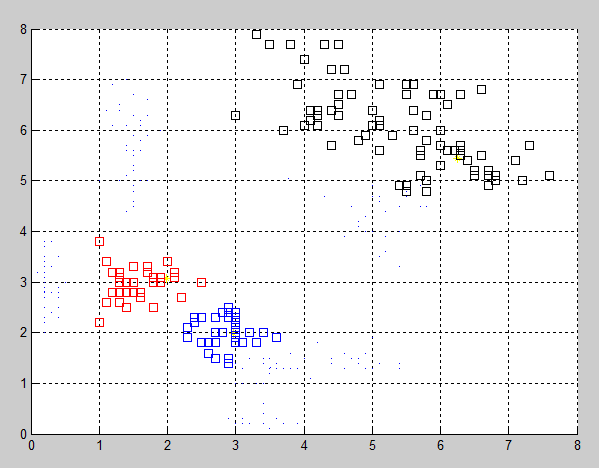
\includegraphics[width=\linewidth]{figure.PNG}
\caption{Clustering Groups}
\end{figure}

\section{RESULT ANALYSIS}
From the figure -1, we can see that we have found  three groups colored red, blue, and black from a randomly chosen centroids and tuning it to perfection until we found the identical set of matrix to represent the clusters. \\


\section{REFERENCES}

[1] Pattern Classification (2nd Edition) by R. O. Duda, P. E. Hart and D. Stork, Wiley 2002\\

\end{document}


